\documentclass{beamer}
\usepackage[orientation=landscape,size=a0,scale=1.4,debug]{beamerposter}
\mode<presentation>{\usetheme{SDSU}}

\title{News Headline Like Title That Catches People's Attention} %It's almost like it's clickbait!
  
\author{\underline{First Author}$^{1,2}$ \and Second Author$^1$ \and Third Author$^2$}

\institute{$^1$San Diego State University, San Diego, CA. $^2$Top National Laboratory, Lab Town, YY. }

\date{\today}

\event{Very Important Conference}

\email{firstauthor@topuniversity.edu}

\website{myresearchsite.com}

\logoleft{\vspace{1cm} \hspace{1cm} 
\includegraphics[height=10cm,keepaspectratio]{SDSUprimary3CrgbRV.png}}

% If you have a second institution you can use \logoright to set the file
% It's ideal to have a high resolution file with transparent background
% Or maybe a professional looking photo of you?
% \logoright{\vspace{1cm} \hspace{1cm} 
\includegraphics[height=10cm,keepaspectratio]{SDSUprimary3CrgbRV.png}}

\begin{document}
	\begin{frame}{}
		\begin{columns}[t]
%%%%%%%%%%%%%%%%%%%%%%%%%%%%%%%%%%%%%%%%%%%%%%%%%%%    First column starts here
			\begin{column}{0.32\linewidth}
				\begin{block}{01 Introduction}
					Nobody wants to read long text in a poster
					\begin{itemize}
						\item It's better to use bullet points
						\item One idea, one bullet point
						\item One bullet point, one sentence
						\item Why is this research important?
						\item What are the goals of this work?
						\item How will those goals be achieved?
					\end{itemize}
				\end{block}
				\vskip1ex % This controls the vertical distance between blocks. Once you've put all the content you'll probably want to finetune these numbers so that your blocks look evenly distributed.

				\begin{block}{02 Methodology}
					Your text goes here

					Maybe you want to write an equation, but remember to keep it simple
					\begin{equation*}
						y = f(x)
					\end{equation*}
					Nothing that may intimidate the reader

				\end{block}
				\vskip1ex

				\begin{block}{03 New Theoretical Tool}
					\begin{columns}
						\begin{column}{.45\linewidth}
							\begin{itemize}
								\item You can use columns to mix text and figures
								\item Expensive numerical integrals
							\end{itemize}
							\begin{equation*}
								\begin{aligned}
									g(\rho) &\sim \int dr \left\{ \left[\Pi_0(\rho,r) \right]^2 + \ldots \right\} \\
									& r^2 \left[ V_c(r) + 3W_c(r) + \ldots \right]
								\end{aligned}
							\end{equation*}
						\end{column}
						\begin{column}{.45\linewidth}
							\begin{center}
								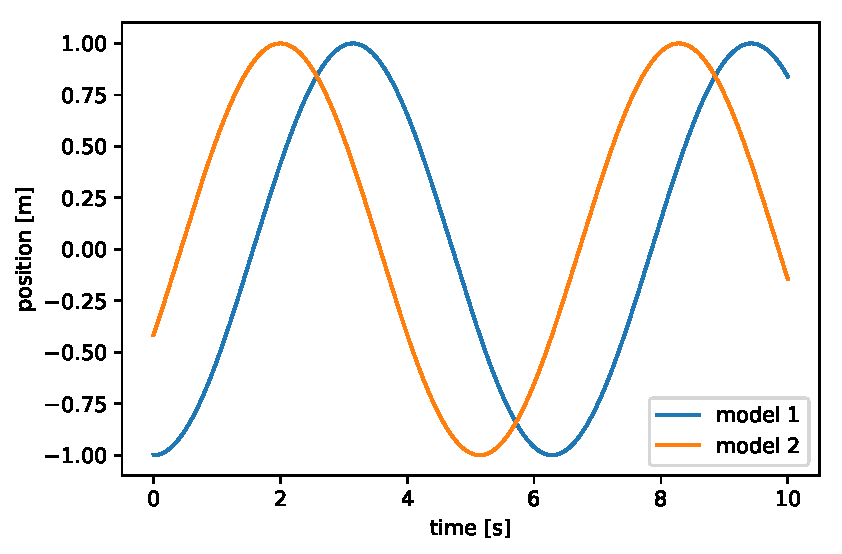
\includegraphics[width=\textwidth]{fig_example.pdf}
							\end{center}
						\end{column}
					\end{columns}

					More text can go bellow the columns that spans the whole block
					\begin{itemize}
						\item Replace with interpolating functions
					\end{itemize}
					\begin{equation*}
						g(\rho) = g_0 + \sum_{i=1}^{M} a_i \left[\tan^{-1}(b_i \rho^{c_i}) \right]^i
					\end{equation*}
				\end{block}
			\end{column}
%%%%%%%%%%%%%%%%%%%%%%%%%%%%%%%%%%%%%%%%%%%%%%%%%%%    Second column starts here
			\begin{column}{0.32\linewidth}
				\begin{block}{04 More Context}
					Want to contrast two things? You can use example and alert blocks
					\vskip2ex
					\begin{columns}
						\begin{column}{.45\linewidth}
							\begin{exampleblock}{Effective interaction}
								\begin{itemize}
									\item Contact coupling parameters
									\item Constrained by Infinite Nuclear Matter properties
									\item Fitted to 130 experimental masses and radii
									\item UNEDF2 as a starting point
								\end{itemize}
							\end{exampleblock}
						\end{column}
						\begin{column}{.01\linewidth}
							\begin{center}
							vs
							\end{center}
						\end{column}
						\begin{column}{.45\linewidth}
							\begin{alertblock}{Realistic interaction}
								\begin{itemize}
									\item Determined by Chiral interactions
									\item Systematic improvement order by order
									\item Fixed for a given order and regulator
								\end{itemize}
							\end{alertblock}
						\end{column}
					\end{columns}
				\end{block}
				\vskip1ex

				\begin{block}{05 Results}
					A good figure can be worth a thousand words
					\begin{center}
						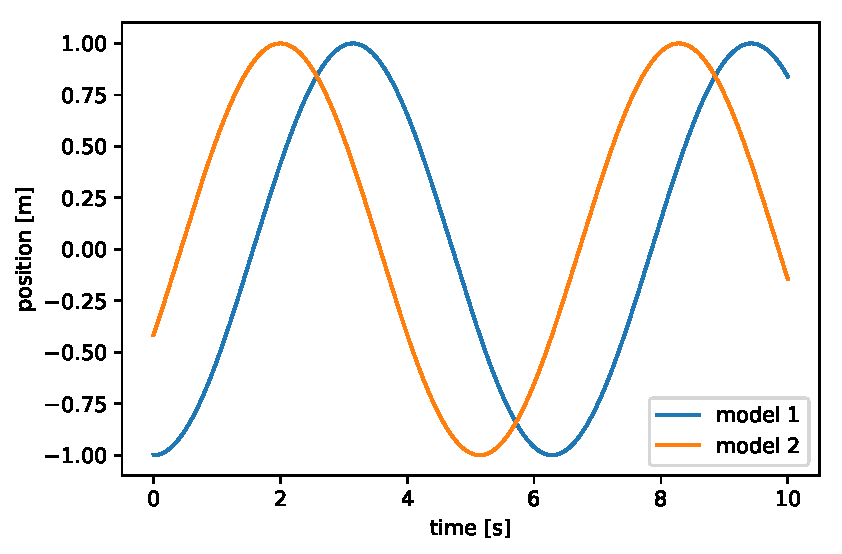
\includegraphics[width=0.75\textwidth]{fig_example.pdf}
					\end{center}
				\end{block}
				\vskip1ex

				\begin{block}{06 Ground Breaking Results}
					\begin{itemize}
						\item Remember to use high resolution figures with transparent background
						\item If you're using \texttt{matplotlib} to generate your figures you can do
					\end{itemize}
					\texttt{plt.savefig(`fig\_example.pdf', format=`pdf', bbox\_inches=`tight', transparent=True)}
				\end{block}
			\end{column}

%%%%%%%%%%%%%%%%%%%%%%%%%%%%%%%%%%%%%%%%%%%%%%%%%%%    Third column starts here
			\begin{column}{0.32\linewidth}
				\begin{block}{07 Can't Believe These Results!}
					Tables can be tricky in a poster, but sometimes that's what works best. Just keep them simple
					\vskip2ex
					\begin{tabular*}{0.91\textwidth}{r@{\extracolsep{\fill}}c l} 
  						\hline
  						constant  & value  & units \\
  						\hline
						$m_p$     & 938.4  & MeV \\
						$m_n$     & 940.1  & MeV \\
						$\hbar c$ & 197.327 & MeV fm \\
 						\hline
					\end{tabular*}
				\end{block}
				\vskip1ex

				\begin{block}{08 Summary}
					\begin{itemize}
						\item Time to wrap things up
						\item Summarize the strengths of your methodology
						\item Summarize your results
						\item What evidence supports our thesis?
						\item What new information can be said based on these results?
					\end{itemize}
				\end{block}
				\vskip1ex

				\begin{block}{09 Outlook}
					\begin{itemize}
						\item What comes next?
						\item Which limitations will be addressed?
						\item Where else can you apply your methodology?
					\end{itemize}
				\end{block}
			\end{column}
		\end{columns}
	\end{frame}
\end{document}
